\documentclass[10.5pt,onecolumn]{jsarticle}

% \AtBeginDvi{\special{pdf:mapfile meiryo.map}}

\newcommand{\dg}{\gt}
% plente3用
\usepackage{wrapfig}
\usepackage{subfig}
\usepackage[dvips,final]{graphicx}
\usepackage{array}
\def\thline{\noalign{\hrule height 1pt}}
\def\tvline{\vrule width 1pt}

% enumerate環境
\usepackage{enumerate}
\usepackage{fancybox}
\usepackage{ascmac}
\usepackage{multirow}
\usepackage{url}

% 余白の設定
\usepackage[top=10truemm,bottom=10truemm,left=20truemm,right=20truemm]{geometry}
% 色
\usepackage[usenames]{color}
% ページ番号なし
\pagestyle{empty}

% フォント
% \usepackage[T1]{fontenc}
% \usepackage[sfdefault]{AlegreyaSans} %% Option 'black' gives heavier bold face
% %% The 'sfdefault' option to make the base font sans serif
% \renewcommand*\oldstylenums[1]{{\AlegreyaSansOsF #1}}
% \usepackage{FiraMono}
% \renewcommand*\familydefault{\ttdefault}
% \usepackage[T1]{fontenc}
% \renewcommand{\bfdefault}{bx}

% 図をはるときの,おまじない.1ページに何個の図がいれれるか
\setcounter{dbltopnumber}{10}
\def\dbltopfraction{.9}%.5
%\def\dblfloatpagefraction{.5}

%%

%%%%%%%%%%%%%%%%%%%%%%%%%%%%%%%%%%%%%%%%%%%%%%%
% 数式中の文字を太字にするコマンド
%
\newcommand{\bd}[1]{\mbox{\boldmath$#1$}}
%%%%%%%%%%%%%%%%%%%%%%%%%%%%%%%%%%%%%%%%%%%%%%%
%%%%%%%%%%%%%%%%%%%%%%%%%%%%%%%%%%%%%%%%%%%%%%%
% 丸囲み文字にするコマンド
%
\newcommand{\maru}[1]{\textcircled{\scriptsize #1}}
%%%%%%%%%%%%%%%%%%%%%%%%%%%%%%%%%%%%%%%%%%%%%%%

\vspace{-5mm}
\title{{\huge{\textbf{村田研究室 卒業研究テーマ}}}}
\author{〜{\it Natural Language Processing Laboratory}〜}
\date{\texttt{}}

\begin{document}
\maketitle
\baselineskip11pt
\cornersize{2}

\vspace{-15mm}
  \section*{\colorbox{black}{\textcolor{white}{{\LARGE 研究室概要}}}}
  %%%
  % old
  %%%
  % 自然言語(Natural Language)とは,普段,人間が話したり書いたりする言葉のことであり,人間がコミュニケーションを取るための最も手軽な方法の一つです.
  % 自然言語を機械によって処理することを自然言語処理と呼びます.
  % % ,自然言語処理技術によって人間と人間,もしくは,人間とコンピュータとのコミュニケーションを促進することが可能となります.
  % 自然言語処理技術の代表例として,「機械翻訳」「情報検索」等があります.
  % 近年は,大規模言語モデル(ChatGPTに代表される生成AIのテキスト処理部分の基盤となるモデル)の登場により,自然言語処理技術の進歩が著しいです.

  %%%
  % new
  %%%
  自然言語処理(NLP)は,文章や会話などの人間の言語をコンピュータで解析・理解・生成する技術であり,近年,急速に進化しています.
  特に,深層学習技術の進展に伴い,これまでの自然言語処理の限界を超える成果が多く生まれています.
  その中でも大規模言語モデル(LLM)は,ChatGPTを代表とする生成AIの基盤技術として注目されています.
  これにより,自然言語処理の応用範囲はさらに広がり,機械翻訳や情報検索だけでなく,要約生成,感情分析,文書生成など,様々なタスクで人間に匹敵する性能を発揮しています.

  % 私たちの研究室では、こうした最新技術を活用し、自然言語の深い理解とそれに基づく応答生成や情報抽出など、次世代の言語処理技術の研究を行っています。特に、ディープラーニングや大規模データを活用した応用研究を通じて、より精度の高い言語処理技術の開発を目指しています。これからの卒業研究では、実世界での自然言語処理の活用を目指したプロジェクトに参加する機会があります。興味のある学生はぜひ、私たちと一緒に未来の言語処理技術の開発に挑戦してみてください。

  \vspace{1mm}
  村田研究室では,特に,{\Large {\dg 音声言語}}(人間が話した言葉を文字化したテキスト)を対象とした研究を行います.
  現在のメイントピックは,「{\dg 人の語りを傾聴するシステムの開発}」と「{\dg 読みやすい字幕を生成するシステムの開発}」です.

  \vspace{-1mm}
  \section*{\colorbox{black}{\textcolor{white}{{\LARGE 研究テーマ}}}}
    \subsection*{\underline{人の語りを傾聴するシステムの開発}}

    \begin{wrapfigure}[10]{r}[32pt]{7cm}
      \vspace{-20mm}
      \begin{center}
        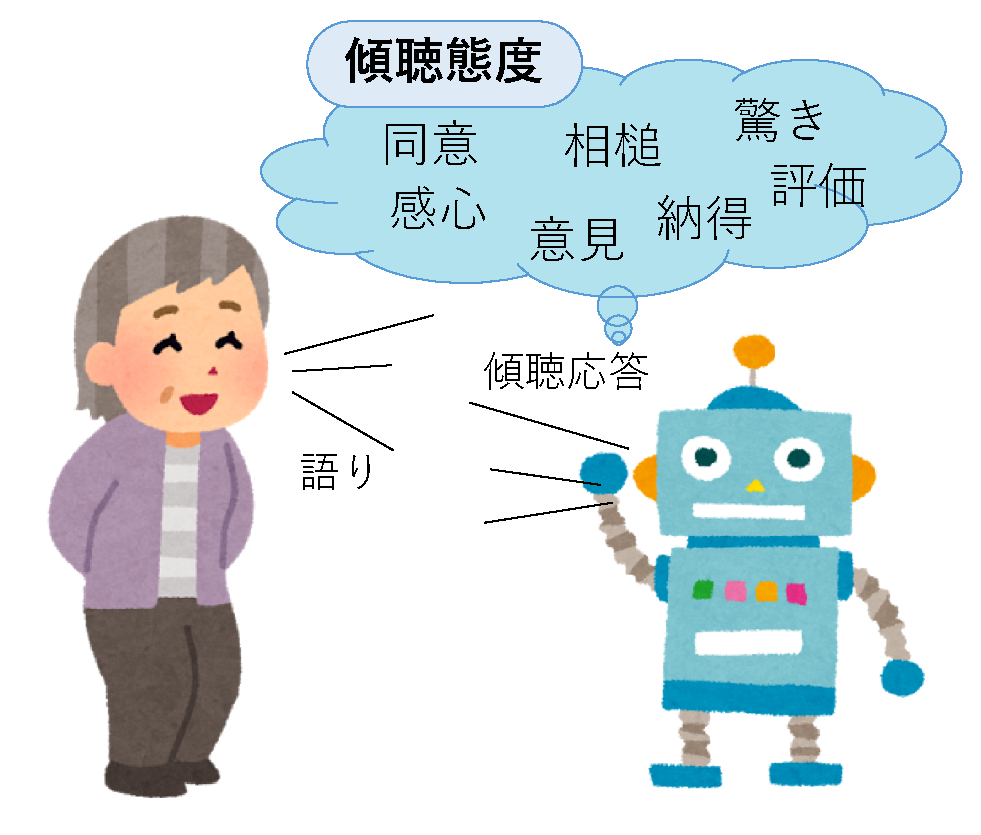
\includegraphics[width=0.3\textwidth]{./pic/robot.eps}\\
        \label{robot}
      \end{center}
    \end{wrapfigure}

    %%%
    % old
    %%%
    % 人間には根本的に語りたいという欲求が備わっています.
    % しかし,話を聞いてくれる人がいつもいるとは限りません...そこで,情報機器に聴き手となってもらいます.
    % 話をきちんと聴いているなと思わせるには,適度に相づちを打ったり,話し手の気持ちに共感したり,褒めたりといった応答を返すことが重要です.
    % これらの応答を返す行為を{\dg 傾聴}と呼びます.
    % 本研究では,人間の話を傾聴するための要素技術の開発を行います.
    % また,それらの技術を統合した傾聴応答システムの実現を目指します.

    %%%
    % new
    %%%
    人間には誰かに話を聞いてほしいという根源的な欲求があります.
    しかし,常に話し相手がいるわけではありません.
    そこで,情報機器が聴き手となり,適切な応答を返すことで,ユーザーに安心感や共感を与えるシステムの開発を目指します.
    傾聴とは,話し手の話に適切なタイミングで相づちを打ち,感情に寄り添う応答を行うことを指します.
    本研究室では,傾聴応答を実現するためのさまざまな要素技術を開発し,最終的にこれらを統合したシステムの構築を目指しています.

    \begin{itemize}
      % old
      % \item[\maru{1}] {\dg 傾聴応答データの分析による傾聴応答に関する知見の獲得}
      % \item[\maru{2}] {\dg 深層学習を用いた傾聴応答タイミングの推定}
      % \item[\maru{3}] {\dg 深層学習を用いた傾聴応答種類の推定,文字列の生成}
      % \item[\maru{4}] {\dg 傾聴応答システムの実現} etc...
      % new
      \item[\maru{1}] {\dg 音声情報と言語情報を併用した傾聴応答タイミングの推定}
      \item[\maru{2}] {\dg ユーザフィードバックに基づく傾聴応答の個人最適化}
      \item[\maru{3}] {\dg マルチモーダルデータを活用した傾聴応答の最適化}
      \item[\maru{4}] {\dg 大規模言語モデルを活用した応答生成の高度化} etc...
    \end{itemize}

    \vspace{-3mm}
    \subsection*{\underline{読みやすい字幕を生成するシステムの開発}}

    \begin{wrapfigure}[10]{r}[32pt]{7cm}
      \vspace{-20mm}
      \begin{center}
        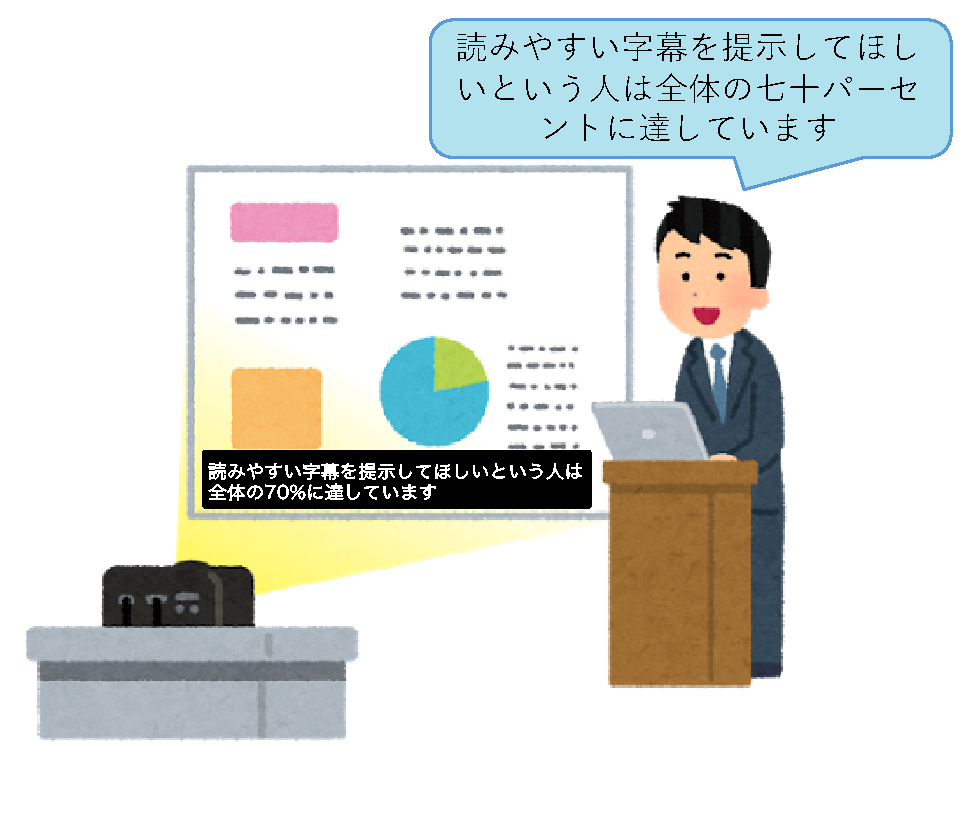
\includegraphics[width=0.4\textwidth]{./pic/transcription.eps}\\
        \label{transcription}
      \end{center}
    \end{wrapfigure}

    %%%
    % old
    %%%
    % 講演等の場で,高齢者や聴覚障害者の方のために字幕を提示する試みは多くなされています.
    % また,スライドを用いた(遠隔を含む)講義・講演においても字幕は有用な情報源です.
    % そこで,より読みやすい字幕を生成・提示することができれば,内容理解の支援に繋がると考えられます.
    % 音声認識により自動で文字起こしされた結果を,字幕自体の読みやすさ,提示方法等を考慮し,読みやすい字幕へ変換して提示することを目指します.

    %%%
    % new
    %%%
    高齢者や聴覚障害者の方々にとって,講演や講義での字幕は重要な情報源です.
    また,スライドを用いた授業やプレゼンテーションにおいても,字幕は聴講者の理解を深める有用な手段です.
    しかし,自動音声認識で生成された文字起こし結果は,必ずしもそのまま読みやすいとは限りません.
    本研究室では,文字起こしされたテキストを整形し,視覚的にわかりやすく表示するためのシステムを開発しています.
    読みやすい字幕の生成を目指し,以下のテーマに取り組みます.

    \begin{itemize}
      % old
      % \item[\maru{1}] {\dg 整形に基づく読みやすい字幕テキストの生成}
      % \item[\maru{2}] {\dg スライド内容との親和性を考慮した字幕テキストの生成}
      % \item[\maru{3}] {\dg 新たな字幕提示方法の提案,提示システムの開発} etc...
      % new
      \item[\maru{1}] {\dg 音声と視覚情報の同期による字幕表示の最適化}
      \item[\maru{2}] {\dg ユーザ個別最適化字幕の生成}
      \item[\maru{3}] {\dg 発話時間と字幕提示時間の差異を埋める字幕提示}
      \item[\maru{4}] {\dg 字幕と感情表現の連携} etc...
    \end{itemize}

    \vspace{-3mm}
    \subsection*{\underline{今年度実施しているテーマ}}
    % 以下は,過去に実施した研究テーマの一例です.

      \begin{itemize}
        \item {\dg 連続的な傾聴応答のタイミングおよび種類の推定}
        \item {\dg 語りの感情情報を利用した傾聴応答の生成}
        \item {\dg 強化学習を用いた字幕テキストの短縮における精度改善}
        \item {\dg 同時音声翻訳モデルにおける訳抜けを利用した短縮字幕生成}
        \item {\dg 意味と音韻を考慮する日本語言語モデルの構築}
      \end{itemize}

    % \vspace{-3mm}
    % \subsection*{\underline{上記以外の研究テーマ}}
    上記以外にも,皆さんからの(言語処理に関する)研究テーマの提案も歓迎します.
    % 以下は,過去に実施した研究テーマの一例です.

    %   \begin{itemize}
    %     \item {\dg 英語発音評価システムの開発}
    %     \item {\dg プレゼンテーション練習システムの開発}
    %     \item {\dg 閲覧ページの要約を表示可能なブラウザの開発}
    %     \item {\dg 思考整理を促す質問文の生成手法の開発}
    %     \item {\dg 文の分割と翻訳可能性の判定に基づく同時通訳システムの開発}
    %     \item {\dg ロボカップ小型リーグにおけるロボットの行動予測}
    %   \end{itemize}

  \vspace{-1mm}
  \section*{\colorbox{black}{\textcolor{white}{{\LARGE メッセージ}}}}

  研究を進めるうえで,言語処理に関する能力(言語学や数学に関する基礎学力,プログラミング能力(主に Python を使用)),また,既存研究を調査・理解する能力等が必要になります.
  これらの能力は研究を根気よく進めていくうえで自然と身についていくものです.
  まずは教員と報連相をしっかり行い,1年を通して集中して取り組める研究テーマを見つけましょう.

\end{document}
